\chapter{Plugin továbbfejlesztése}

Ebben a fejezetben ismertetem a beépülő modulon végzett továbbfejlesztéseket melyeket a mesterképzés során végeztem. 

\section{Fejlesztés céljai}

A fejlesztés során hozott alkalmazott megoldások áttekintése előtt érdemes végigvenni, hogy mik is voltak a fejlesztés fő céljai és mi volt ezeknek a motivációja.

\subsection{Funkcionális dekompozíció transzformálása}
Egy rendszert állapotait és állapotváltásait le lehetne modellezni egy mindent tartalmazó állapotgéppel, párhuzamos régiókkal és egyéb modellezési megoldásokkal. Ahogy a modell mérete nő a funkcionalitást érdemes feldarabolni és részenként modellezni. Ez nem csak az áttekinthetőséget segíti, de megkönnyíti a modellen való csapatmunkát is a mérnökök számára hiszen a szétbontott részeket külön, egymástól független lehet modellezni, majd ezeket összekapcsolni.

Szerencsére a Gamma erre a problémára is megoldást kínál, támogatja az állapot dekompozíció modellezését és formális verifikációját.

\subsection{Eredmények megjelenítése}
Fontos kérdés, hogy a formális verifikáció eredményét milyen formában kívánjuk megjeleníteni a mérnökök számára. A plugin eddigi verziója csak arra a kérdésre tudott választ adni, hogy teljesülnek-e a modellel szemben támasztott megkötések vagy sem.

Az \uppaal és a Gamma is képes sokkal részletesebb választ adni. Ezt a Gamma Back-annotation formájában teszi azaz a verifikációban előállt időzítések és lépéseket visszavezeti az eredeti modellbe. Ehhez a Gamma egy elég jól értelmezhető nyelvtant definiál, azonban a SysML-t jellemzően rendszermérnökök használják akik inkább a diagramokat mint a szöveges leírásokat preferálják általában.

A Back-annotationt úgy is lehet interpretálni mint lépések egy sorozatát, amelyek szinkron esetben egymást jól meghatározható sorrendben követik. Ezt leginkább szekvencia diagramokon lehet ábrázolni. Ezen felül ami miatt még a szekvencia diagram tűnik a legkézenfekvőbb megjelenítési megoldásnak az a MagicDraw, illetve a Cameo Simulation toolkit. Ez ugyanis képes szimulációt rögzíteni szekvencia diagramok formájában (\refstruc{fig:md-cameo-rec})) és ezeket újra lejátszani. A cél tehát olyan szekvencia diagramok előállítása úgy minthogyha a szimulátort használva találtuk volna meg a hibautakat, így ezekről nem csak egy jól áttekinthető megoldást kapunk szekvenciák formájában, hanem ezek szimulálhatók is lesznek Cameo Simulation Toolkit segítségével.

\begin{figure}[!ht]
	\centering
	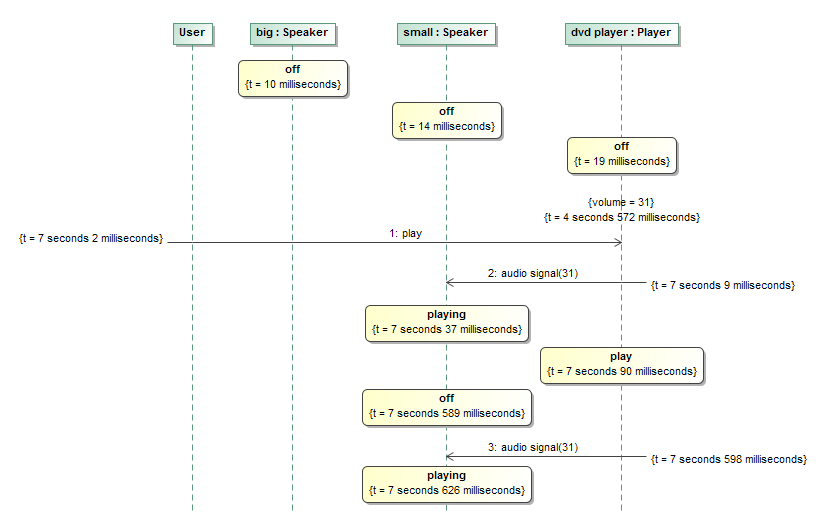
\includegraphics[width=140mm, keepaspectratio]{figures/contribution/md-cameo-rec.png}
	\caption[]{Rögzített szimuláció szekvencia diagramon\footnotemark}
	\label{fig:md-cameo-rec}
\end{figure}

\footnotetext{Forrás: https://docs.nomagic.com/display/CSTD184/Recording+simulation+as+a+Sequence+diagram}

\subsection{Követelmények definiálása}

A formális verifikáció elvégzéséhez a modelleken felül meg kell tudnia a felhasználónak azokat a kérdéseket melyekre választ szeretne kapni a modell ellenőrzése során. Ezek jelen esetben a "Kerülhet-e a rendszer adott állapotba" illetve "Adott állapotból el tud-e jutni egy másikba" típusúak jellemzően. Az \uppaal-ban ezeket temporális logikai kifejezések segítségével tudjuk megtenni \uppaal Queryk formájában ezért ezeket az ellenőrzés során elő kell állítanunk.

Eredetileg szándékoztam erre egy saját nyelvtant is fejleszteni, de a Gammához időközben készült egy úgynevezett \emph{Property Language} és ez ennek az \uppaal-ra transzformáló funkciója és végül ezt használtam fel.

\subsection{Validáció}

A fejlesztés során hozott számos döntés megköveteli, hogy a modellekre vonatkozzanak bizonyos jól-formáltsági kényszerek. Ezek egy része a Gammából örökölt. Például a \emph{Property Language} egy komponensen belül egy állapotra a régión keresztül tudunk hivatkozni (\emph{[component]+.region.state}). Ebből következik, hogy a régióknak a MagicDraw modellben nevet kell adni, illetve, hogy ezek egyediek legyenek egy állapottérképen belül.

A dolgozat célja egy validációs szabálykészlet létrehozása ami segít a felhasználóknak az eszköz helyes használatában.

\newpage

\section{Gamma UML profil}

A dolgozat elkészítéséhez pusztán a SysML nyelv nem volt elegendő ugyanis szükséges volt  a modellben is eltárolni  bizonyos információkat, mint például az ellenőrizendő követelmények, a Back-annotation, vagy éppen, hogy milyen kompozit szemantikát kívánunk érvényesíteni az adott modellekre.

Ezek információk modellezhetőségéhez készítettem egy MagicDraw profilt. Ez alapvetően három részből áll:

\begin{itemize}
	\item Kompozit szemantika
	\item Check modell
	\item Back-annotation modell
\end{itemize}

Az UML profil érdekessége, hogy tartalmazásokat csak megkötés szintjén \emph{Customization}on keresztül tudunk megadni. UML profil diagramon csak öröklést és \emph{tag}eket van lehetőségünk definiálni.



\subsection{Kompozit szemantika}

A Gamma háromféle komponens végrehajtási szemantikát biztosít a felhasználók számára. Ugyan ezt implicit módon is meg lehet határozni, például a kommunikáció típusából, mégis fontos lehet ezek egyértelmű jelölése. Ezért az UML profil (\refstruc{fig:comp-prof}) a SysML nyelvet kiegészíti néhány sztereotípiával melyek segítségével explicit jelölhetők, hogy milyen szemantikát szeretne a felhasználó érteni Blokkjain.

\begin{figure}[!ht]
	\centering
	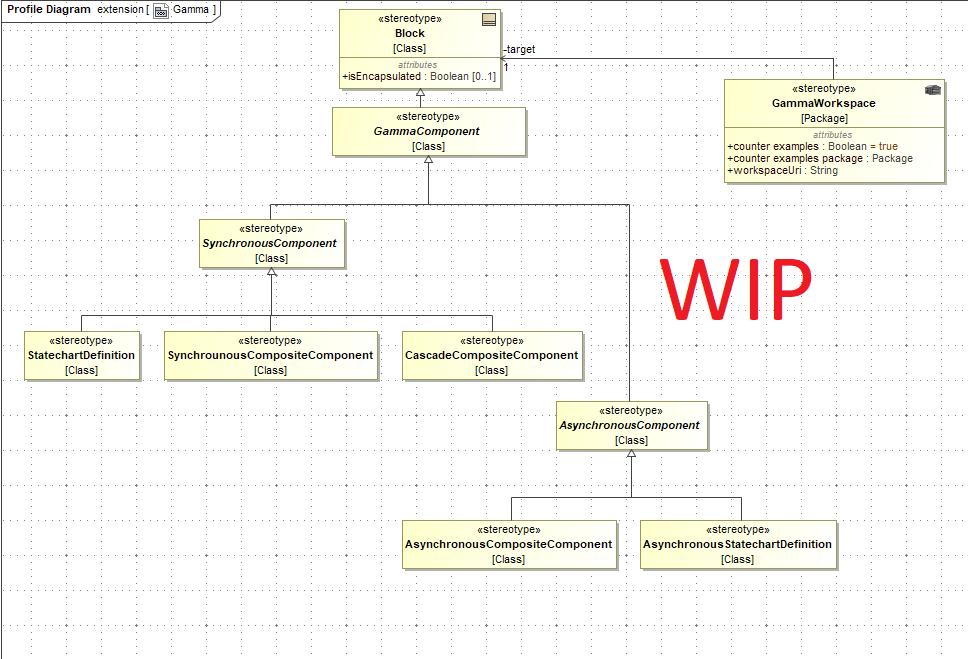
\includegraphics[width=150mm, keepaspectratio]{figures/contribution/profile.png}
	\caption{Szinkron, asszinkron szemantikát támogató UML profil}
	\label{fig:comp-prof}
\end{figure}

A sztereotípiák leszármaznak a Block sztereotípiájából, így lényegében lecserélik azt. Ennek előnye hogy szintaktikailag is asszinkron és szinkron blokkok fognak megjelenni a modelljeinkben. Viszont van egy nagyon nagy hátulütője is mégpedig az, hogyha már meglévő modelleken szeretnénk használni az eszközt ezekhez hozzá kell nyúlni, amihez például elosztott környezetben nem biztos, hogy egyszerű. Ami mégis elfogadhatóvá teszi ezt a plugin jelenlegi iterációjának kapcsán az az őrfeltételek és az akciókra vagy akár az interfészekre vonatkozó megkötések amik - sajnálatos módon - jó eséllyel megkövetelik a modell módosítását.

Egy alternatív megoldás az lehetne, hogy a sztereotípiákat valamilyen él például \emph{Dependency} segítségével rendeljük az egyes komponens definíciókhoz, vagy akár partokhoz. Ez megoldást nyújthat arra a problémára is, hogyha a modell egyes részei külső könyvtárból jönnek, vagy nincs hozzáférésünk hozzájuk.


\subsection{Check modell}

Ahhoz, hogy a formális verifikáció végrehajtható legyen ki kell választani, hogy milyen modelleket szeretnénk ellenőrizni és ezeken milyen követelményeket. Az formális verifikációt modell elemeken keresztül lehet paraméterezni.

Az elképzelés szerint a felhasználó \emph{Workspace}eket hoz létre. Ezek hivatkoznak a felhasználó számítógépén egy könyvtárra melyet az infrastruktúra sajátosságából adódó háttértárra kimentendő modelleket tárolására használok. Ezen felül rajta keresztül kell behivatkozni az ellenőrizendő modellt a projektből.

A modell transzformációk során \emph{Trace}k keletkeznek. Ezek alapján lehet visszakeresni, hogy mely a MagicDraw - Gamma transzformáció során milyen leképzések történtek. Ezek valójában UML propertyk egy \emph{Class}on belül melyeknek a neve egy azonosító amivel a Gamma modell egy kisorosított XMI fájlban lévő elemei vannak hivatkozva. A \emph{property}kből egy \emph{Trace} él mutat a megfelelő MagicDraw elemekre. A kisorosított XMI ugyan ezen \emph{Class} modell elemekhez mint \emph{Comment} vannak hozzárendelve, innen lehet őket kiolvasni.

A követelményeket \emph{GammaProperty} segítségével lehet megadni a Gamma által definiált Property nyelvtan segítségével. Az ezek ellenőrzéséből származó Back-annotaion modellek is a \emph{Workspace}ben helyezkednek el. A modell elemei a következők:
%TODO Update
\begin{itemize}
	\item \textbf{GammaWorkspace} \newline
	Transzformációk és ellenőrzések kezelésére szolgáló MagicDraw projektben tárolt modell.
	\newline
	\textit{Attribútumok:}
	\subitem Target: InstanceSpecification[1]: transzformálandó modell
	\subitem WorkspaceUri: String: egy elérési út a felhasználó egy könyvárához
	\subitem Counter examples: Boolean: Back-annotation engedélyezése
	
	\item \textbf{GammaCheck} \newline
	\emph{GammaProperty}k konténere
	
	\item \textbf{GammaProperty} \newline
	Egy a modellel szemben támasztott követelmény a saját nyelven
	\newline
	\textit{Attribútumok:}
	\subitem body: String[1]: saját nyelven írt kifejezés

	\item \textbf{GammaWorkspaceFile} \newline
	Hivatkozás egy Gamma modellre a háttértáron. A modell elem neve a fájl elérési útja.
	
	\item \textbf{MD2G\_Trace} \newline
	Egy megfeleltetés a MagicDraw és Gamma modellek között. A MagicDraw elemre egy Trace él mutat, a Gammabeli modell elem pedig EMF hivatkozás formájában kerül tárolásra.
	\newline
	\textit{Attribútumok:}
	\subitem URIFragment: String[1]: hivatkozás EMF-es modell elemekre
	
	
\end{itemize}

\subsection{Back-annotation modell}
A back-annotation modell feladata visszacsatolni az eredeti modellbe a valamilyen külső, jellemzően szimulátorból származó időzítési adatokat. A Gamma is készít egy ilyen modellt. A megoldás amit kidolgoztam Gamma modell egy MagicDraw specifikus változatának létrehozásából és egy Gamma-MagicDraw transzformáció megtervezéséből és megvalósításából állt. Az UML profil egy szakterület specifikus nyelvet definiál. Elemei pedig a következők:

\begin{itemize}
	\item \textbf{ExecutionTrace} \newline
	Egy kompozit komponens végrehajtása. \textit{Steppeket} azaz lépéseket tartalmaz, illetve a végrehajtás végén állhat egy lépésekből álló ciklus.
	\newline
	\textit{Attribútumok:}
	\subitem component: InstanceSpecification[1]: kompozit komponens példánya a modellben
	\subitem steps: Step[1..*]: lépések
	\subitem cycle: Cycle[0..1]: lépésekből álló ciklus amire a végrehajtás futhat
	
	\item \textbf{Step} \newline
	A végrehajtás egy lépése. Két részből áll egy \textit{Act} részből, ami a végrehajtódott műveleteket írja le és egy \textit{Assert} részből, ami a lépésben elért állapotot írja le.
	\newline
	\textit{Attribútumok:}
	\subitem actGroup: ActGroup[0..1]: műveletek konténere
	\subitem assert: Assert[1]: lépés során beálló állapotok
	
	\item \textbf{ActGroup} \newline
	\textit{Actok} konténere a \textit{Steppen} belül. Csak áttekinthetőségre szolgál.
	\newline
	\textit{Attribútumok:}
	\subitem acts: Act[0..*]: műveletek konténere
	
	\item \textbf{Act} \newline
	Absztrakt sztereotípia. Egy végrehajtott művelet.
	
	\item \textbf{ComponentSchedule} \newline
	Komponensen egy kör végrehajtása (üzenetek kiolvasása az üzenetsorokból, állapotok léptetése)
	
	\item \textbf{TimeElapse} \newline
	Végrehajtás várakoztatása bizonyos ideig.
	\newline
	\textit{Attribútumok:}
	\subitem value: Integer: várakozás ideje milliszekundumban
	
	\item \textbf{RaiseEventAct} \newline
	Egy esemény elküldése a komponens példánynak.
	\newline
	\textit{Attribútumok:}
	%TODO ez itt biztosan válozik majd
	\subitem referencedAction: Behavior: eseményt küldő viselkedés.
	
	\item \textbf{InstanceState} \newline
	Absztrakt. Az egyes példányok, partok állapotainak leírása.
	\newline
	\textit{Attribútumok:}
	\subitem referencedPart: PartProperty: hivatkozott komponens példány
	
	\item \textbf{InstanceVariableState} \newline
	Egy változónak egy állapota.
	\newline
	\textit{Attribútumok:}
	\subitem referencedVariable: Property: hivatkozott változó
	\subitem value: ValueSpecification: hivatkozott változó értéke
	
	\item \textbf{InstanceStateConstant} \newline
	Az állapot gép egy állapota.
	\newline
	\textit{Attribútumok:}
	\subitem referencedState: State: hivatkozott állapot konstans
\end{itemize}

A \refstruc{fig:contribution-trace-profile} az UML profilt, a \refstruc{fig:contribution-trace-customization} pedig ennek a customizationjét mutatja.

\begin{figure}[!ht]
	\centering
	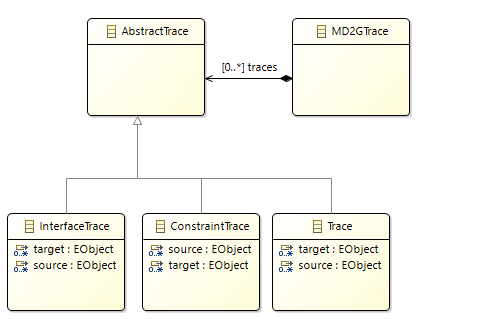
\includegraphics[width=90mm, keepaspectratio]{figures/contribution/trace-model.png}
	\caption{Back-annotation UML profilja}
	\label{fig:contribution-trace-profile}
\end{figure}

\begin{figure}[!ht]
	\centering
	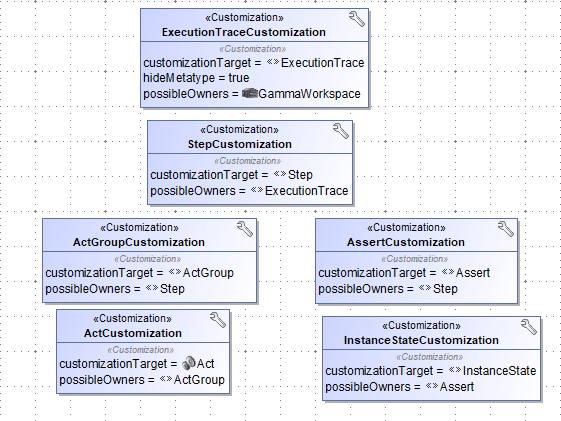
\includegraphics[width=90mm, keepaspectratio]{figures/contribution/trace-profile.png}
	\caption{Back-annotation customization modellje}
	\label{fig:contribution-trace-customization}
\end{figure}
 
 \newpage


\section{Kompozíciók transzformációja}

Egy nagy komplex rendszert célszerű nem egyben, hanem részekre bontva modellezni majd a részek egymáshoz illesztéséből, komponálásából képezni a teljes rendszert. Állapottérképek dekomponálását azaz részekre bontását a Gamma is támogatja. A kihívás a SysML és a Gamma közötti megfeleltetések megválasztása oly módon, hogy a szemantika ne sérüljön. A megfeleltetés két szempontól kell vizsgálni, egyszer az elemek tartalmazási hierarchiái szerint, egyszer pedig a köztük modellezett kommunikáció szerint.



\subsection{Struktúra megfeleltetése}
A Gammában nyelvi szinten elkülönül az állapottérkép (StatechartDefinition) és a kompozit komponens (Composite Component) fogalma. Állapottérképek a modell hierarchia gráfjában a levelekben helyezkednek el. SysML esetében a minden Blokknak lehet viselkedése, jelen esetben állapottérképe. A megfeleltetés elvégzéséhez megkötést fogalmaztam meg mely kétféle blokkot enged meg. A viselkedéssel rendelkező blokkokat és azokat amelyek nem tartalmazhatnak viselkedést csak Part Propertyket. Tehát állapottérképek ebben a modellben is csak levelekben lehetnek.

\begin{figure}[!ht]
	\centering
	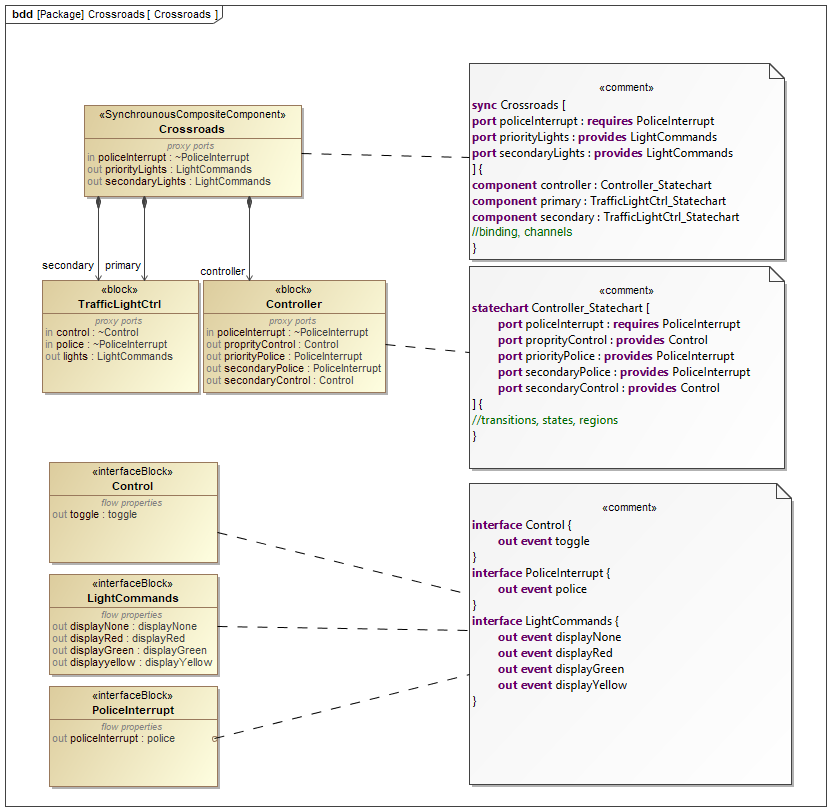
\includegraphics[width=140mm, keepaspectratio]{figures/contribution/md2g.png}
	\caption{Struktúra megfeleltetése}
	\label{fig:md2g}
\end{figure}

Az érdekes kérdés lehet, hogy ha egy magasabb szintű blokknak mégis lehetne viselkedése, azt szemantikailag hogyan kezelhetnénk. Elképzelhető olyan értelmezés, hogy ez a magas szintű állapottérkép a dekomponált részek együttes viselkedését írja le. Ez lehetőséget adna arra, hogy a magasabb és az alacsonyabb szintű viselkedés halmazt összehasonlítsuk működés szempontjából és ha nincsenek szinkronban akkor tervezési hibaként értelmezzük. Így a magasabb hierarchia szintek tulajdonképpen validálnák az alacsonyabb szinteket. Ennek a lehetőségnek a komolyabb kifejtése azonban nem célja a dolgozatnak.

\subsection{Kommunikáció megfeleltetése}

A Gammában a komponensek kommunikációja kimondottan az eseményvezérelt állapot alapú rendszerek sajátosságain alapul, azonban SysML-ben a kommunikáció leírása sokkal általánosabb és többféle módon is modellezhető. Éppen ezért a feladat elvégzése során az események és az interfészek modellezésére megkötéseket kellett megfogalmazni.
Az egyik ilyen megkötés szerint a portokban interfész blokkokat kell tipizálniuk és szinkron szemantika esetében operációkat definiálni, asszinkron esetben pedig szignálokkal tipizált \emph{Flow Property} formájában fel kell tüntetni milyen szignálok fogadására képes a blokk.

Az eseményeknek mindig specifikálniuk kell, hogy melyik porton várják az operáció hívását vagy szignál érkezését. Ez igaz az akciókra az ő esetükben azt kell specifikálni, hogy milyen porton keresztül történjen a küldés.

Portok közül csak a \emph{Proxy} portok támogatottak. Proxy portok iránya származtatott a \emph{Flow property} irányokból amik keresztül mehetnek rajta. Az irány az \emph{isConjugated} flag igazra állításával változtatható.

\section{CTL nyelvtan}

\section{Back-annotation transzformációja}

A Back-annotation egy általában szimulátor által biztosított időzítési adatok visszacsatolása az eredeti modellbe. Ahhoz, hogy MagicDrawban is el tudjuk tárolni ezeket az adatokat létre kellett hoznom egy UML profilt ami a Back-annotation modell metamodelljeként fog szolgálni.

A transzformáció iránya itt megfordul nem MagicDraw modellekből állítok elő Gamma modelleket hanem épp fordítva Gamma modelleket transzformálok MagicDraw modellekké.



\section{Szimuláció}

\section{Validáció}

\section{Példa} %TODO TBD

Ebben az alfejezetben bemutatom az eszköz használatát egy példamodellen. Ez a modell a Gamma tutorial csomagjában lévő közlekedési lámpákat tartalmazó modelljének SysML-be átemelt változata. A példán ismertetése közben bemutatom a az eszköz által támogatott modellezési módszertant is.

\subsection{A példamodel}

A modell három komponensből áll (\ref{fig:Crossroads} ábra): két a lámpákat irányító (\emph{primary}, \emph{secondary}) és egy az ezeket szinkronban tartó \emph{Controller} komponensből. A rendszernek van két kimeneti portja amellyel a két közlekedési lámpa jelzéseit tudja változtatni és rendelkezik egy bemeneti porttal amelyen keresztül a rendőrség \emph{Interrupted} ("Sárga villogó") állapotba tudja állítani a rendszert illetve vissza is tudja állítani a normál állapotba, ahol a piros - zöld - sárga jelzések váltakoznak a két lámpán mégpedig egymásnak ellentétesen.

\begin{figure}[!ht]
	\centering
	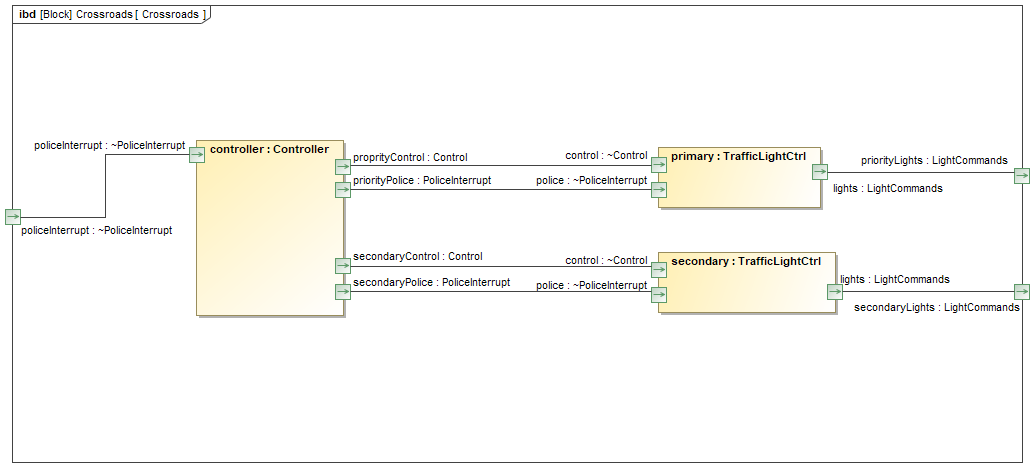
\includegraphics[width=15cm, keepaspectratio]{figures/contribution/Crossroads.png}
	\caption{Az útkereszteződés SysML modellje}
	\label{fig:Crossroads}
\end{figure}

A rendszer három interfészt definiál (\ref{fig:Interfaces} ábra): \emph{PoliceInterrupt}, \emph{Control}, \emph{LightCommands}. Ezek mindegyike \emph{Interface Block}ként kell, hogy megjelenjen a modellben, és minden az állapottérképeken használt \emph{Signal}hoz fel kell venni egy \emph{Flow Property}-t a megfelelő iránnyal. Jelen esetben ez a következőként jelenik meg. A \emph{Control} interfész tartalmaz egy \emph{Flow Property}-t \emph{out}, azaz kimenő iránnyal és egy 'toggle' nevű \emph{Signal}lal van tipizálva. Ez azért fontos mert az állapottérképen ezeket a \emph{Signal}okat kell majd használni. A \emph{LightCommands} négy kimenő \emph{Property}t tartalmaz. Ezek a \emph{displayNone}, \emph{displayRed}, \emph{displayGreed} és \emph{displayYellow} szignálokkal vannak tipizálva. A \emph{PoliceInterrupt} interfész csak egy \emph{Property}t tartalmaz \emph{out} iránnyal a \emph{police} szignálhoz.

\begin{figure}[!ht]
	\centering
	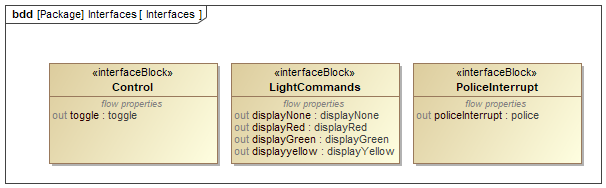
\includegraphics[width=15cm, keepaspectratio]{figures/contribution/Interfaces.png}
	\caption{Interfészek a modellben}
	\label{fig:Interfaces}
\end{figure}

Most, hogy már az interfészek és a portok le vannak modellezve el ezeket fel lehet használni az állapottérképek leírásához. A modell két állapottérképet definiál egyet a két lámpa controllerjéhez (\emph{LightCtr}-hez) és egyet a \emph{Controller}hez.

Tekintsük előbb a \emph{Controller} állapottérképére (\ref{fig:ControllerSM} ábra). Az állapotgép egy kompozit állapotból és ennek négy belső állapotából áll. \emph{Police Interrupt} hatására az állapotgép kilép a kompozit állapotból mindkét \emph{PoliceInterrupt} típusú portján küld egy-egy \emph{policeInterrupt} jelet, majd visszatér ugyan ebbe az állapotba. Amelyben a \emph{History State} miatt abból az állapotba kerül vissza amiben a kilépés előtt volt.

\begin{figure}[!ht]
	\centering
	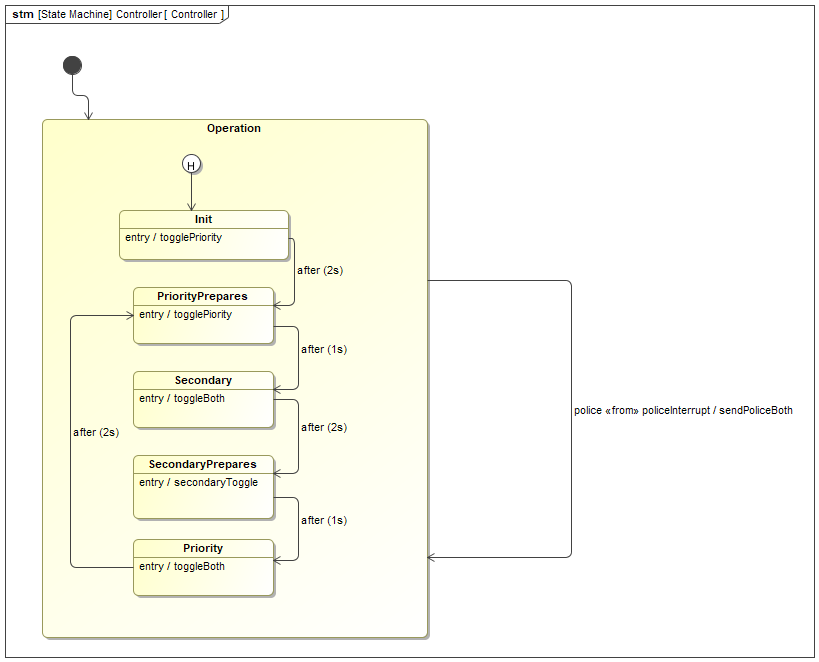
\includegraphics[width=12cm, keepaspectratio]{figures/contribution/ControllerSM.png}
	\caption{Controller állapotai}
	\label{fig:ControllerSM}
\end{figure}

Ami ennek az állapot átmenetnek a modellezése kapcsán izgalmas az \emph{Signal} küldésnek a módja. A plugin jelenlegi formájában ezt Activity diagrammal kell leírni \emph{Send Signal} akciók használatával. Ez jelen esetben egy két akciós \emph{Activity}t fog eredményezni, amelyben sorban a megfelelő portokon elküldésre kerülnek a szignálok (\ref{fig:activity} ábra).  A \emph{togglePriority}, \emph{secondaryToggle} és \emph{toggleBoth} \emph{entry action}ok hasonlóan vannak modellezve.

\begin{figure}[!ht]
	\centering
	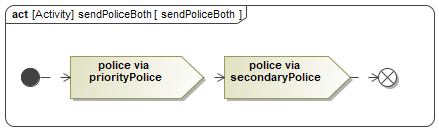
\includegraphics[width=12cm, keepaspectratio]{figures/contribution/sendPoliceBoth.png}
	\caption{\emph{Signal}ok küldése Activityel}
	\label{fig:activity}
\end{figure}

Amiről ennek az állapottérképnek a kapcsán még érdemes lehet beszélni ezek a bizonyos idő elteltével tüzelő átmenetek. Ezek a modellben \emph{Time Event}ként jelennek meg. Fontos hogy ezeknek a \emph{relative} attribútumát igazra kell állítani, hisz ez jelenti azt, hogy a forrás állapotba való belépéstől kell számítani az időt.

A teljesség kedvéért vizsgáljuk meg a másik állapottérképet is (\ref{fig:LightCtrlSM} ábra). Ez két kompozit állapotból áll. A \emph{Normál} a szokásos működést jelenti és a \emph{Red}, \emph{Green}, \emph{Yellow} állapotokból áll melyek a beérkező toggle szignálok hatására váltakoznak.
Az \emph{Interrupted} állapot a rendőrség által előidézett "sárga villogó" állapotot jelenti. Ebben a \emph{BlinkingYellow} és a \emph{Black} állapotok váltakoznak 500 milliszekundumonként.  

\begin{figure}[!ht]
	\centering
	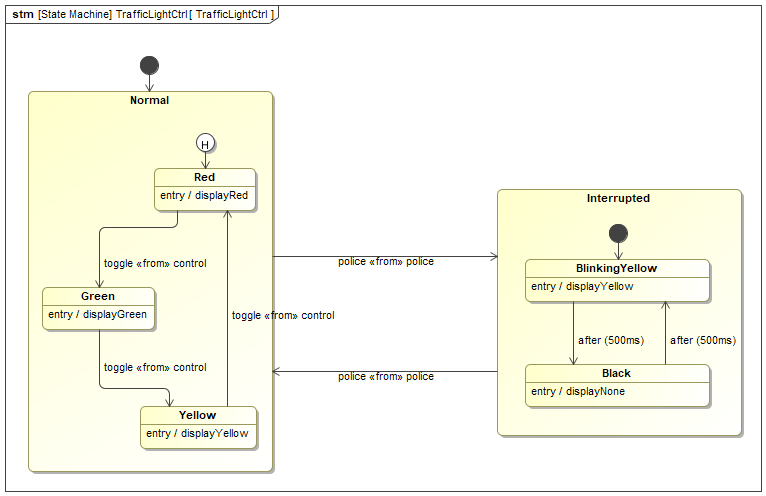
\includegraphics[width=12cm, keepaspectratio]{figures/contribution/TrafficLightCtrlSM.png}
	\caption{\emph{TrafficLightCtrl} állapottérképe}
	\label{fig:LightCtrlSM}
\end{figure}


\subsection{Transzformációk végrehajtása}

A modell összerakásánál egy dolog még nem lett lemodellezve, mégpedig, hogy melyik komponenst szemantikát szeretnénk alkalmazni. Jelen esetben a szinkron szemantikát szeretnénk. Ehhez jelen esetben elegendő a gyökér elem \emph{Block} sztereotípiáját a specifikusabb \emph{SynchronousCompositeComponent}re cserélni.
Most, hogy a komponens szemantika specifikálva van a modellek transzformálhatók és ellenőrizhetők.

Első lépésként létre kell hozni egy \emph{GammaWorkspace}t. Ez a modell elem fogja tárolni az ellenőrzés során szükséges adminisztrációs objektumokat. Azonban meg kell nevezni egy könyvtárat is a háttértáron amit ideiglenes fájlok tárolására fog a plugin használni. Ehhez egy \emph{Workspace Uri}t kell megadni ami egy abszolút elérési út egy tetszőleges könyvtárhoz. Az ellenőrizendő modellt a \emph{Target} mező megadásával lehet specifikálni.

\begin{figure}[!ht]
	\centering
	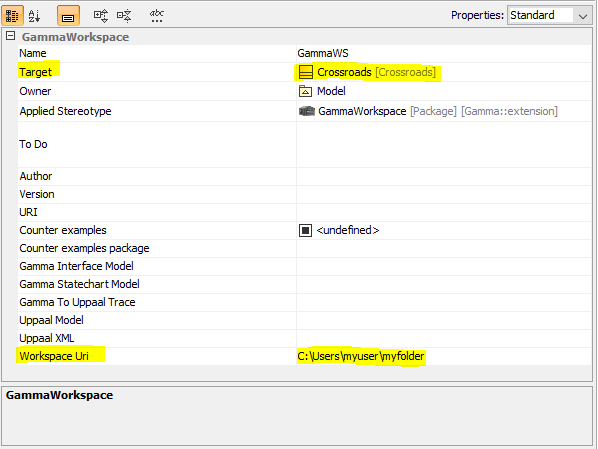
\includegraphics[width=7cm, keepaspectratio]{figures/contribution/GammaWS.png}
	\caption{\emph{GammaWorkspace} specifikációja}
	\label{fig:GammaWS}
\end{figure}


A kötelező mezők specifikálása után a \emph{Gamma Workspace}n nyitott gyorsmenüben a \emph{Gamma Transformation} menüpont alatt található akciók segítségével tudjuk a transzformációkat végrehajtani (\ref{fig:gamma-tra}). Az egymással függésben lévő lépések akkor válnak aktívvá, hogyha a bemenetük már előállt.

\begin{figure}[!ht]
	\centering
	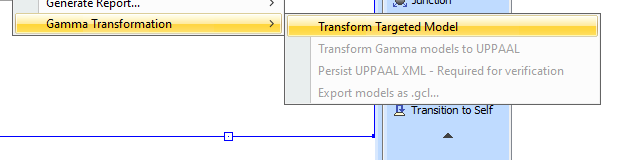
\includegraphics[width=10cm, keepaspectratio]{figures/contribution/GammaTransformation.png}
	\caption{Gyormenü elérése a transzformációkhoz}
	\label{fig:gamma-tra}
\end{figure}

Az akció végrehajtását követően két dolog történik. Először is megjelenik két \emph{GammaModel} sztereotípiával ellátott osztály elem, a transzformált interfészeknek és a komponenst modelleknek illetve állapotgépeknek. Másfelől a \emph{GammaWorkspace} \emph{Gamma Statechart Model} és a \emph{Gamma Interface Model} mezők ezekre fognak mutatni. A letranszformált modellek ezekhez a sztereotipizált osztályokhoz XMI formátumban kommentek formájában hozzá lesznek rendelve innen lehet őket \emph{EMF Resource}okba visszaolvasni amennyiben erre szükség van, így nem kell újra letranszformálni a modelleket.

Az osztályok belsejében továbbá létrejön jó pár \emph{property}. Ezek csomópont hivatkozások az XMI fájlok egyes elemeire. Belőlük pedig \emph{Trace} élek futnak melyek MagicDraw elemekre mutatnak. Ez az a visszakövethetőségi modell melynek segítségével tudjuk, hogy melyik Gamma elem milyen MagicDraw elemekből állt elő. Ezt \aref{fig:traces} ábra szemlélteti, ahol a \emph{Traced element} egy származtatott oszlop a \emph{Trace} élek cél elemei.

\begin{figure}[!ht]
	\centering
	\includegraphics[width=10cm, keepaspectratio]{figures/contribution/Traces.png}
	\caption{Elemek visszakövethetősége MagicDrawban (részlet)}
	\label{fig:traces}
\end{figure}

Következő lépés a az UPPAAL EMF speficikus modelljének előállítása  ez ehhez tartozó \emph{trace}kkel együtt amelyeket a Gamma majd a back-annotation előállításához használ majd. Ezeket a mostmár aktív "Transform models to UPPAAL" akció végrehajtásával tudjuk megtenni. Hasonlóan ez előbb szemléltetettekhez létrejön két sztereotipizált osztály egy az UPPAAL modellnek egy pedig az UPPAAL - Gamma \emph{traceknek}. A modellek ugyan úgy mint az előbb XMI formátumban az elemekhez lesznek kapcsolva. Ebben az esetben nem fognak \emph{property}k megjelenni hiszen ezek a modellek tulajdonképpen nem függnek a MagicDraw modelltől hanem funkcionálisan a Gamma részei.

Az eddigiekben nem volt szükség a háttértárra sorosítani, minden a MagicDraw modell belsejében került tárolásra. Azonban a következő lépés már használni fogja a behivatkozott könyvtárat is. Ez az utolsó lépés amit el kell végeznünk ahhoz, hogy olyan leírás álljon elő amit már az UPPAAL ellenőrzője be tud olvasni. Erre a \emph{Persist UPPAAL XML akció szolgál}. Ez szintén létrehoz egy sztereotipizált osztály elemet ez azonban már nem a \emph{GammaModel} hanem a \emph{GammaWorkspaceFile} sztereotípiát fogja megkapni. Ez utal arra, hogy ez egy külső hivatkozás (\ref{fig:gwsfinal} ábra).

\begin{figure}[!ht]
	\centering
	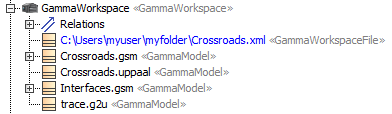
\includegraphics[width=10cm, keepaspectratio]{figures/contribution/gwsfinal.png}
	\caption{Workspace tartalma a transzformációk után}
	\label{fig:gwsfinal}
\end{figure}

Léteznek bizonyos felhasználási módok, hogy ezeket a modelleket MagicDraw-n kívül szeretnénk használni. A modelleket az \emph{Export models as .gcl...} akció végrehajtásával tudjuk kimenteni. Ezek a Gamma nyelvtanára fognak sorosodni.
A korábban bemutatott interfészek például ilyen formában fognak megjelenni:

\begin{lstlisting}
	package Interfaces
	interface LightCommands {
		out event displayNone
		out event displayRed
		out event displayGreen
		out event displayYellow
	}
	interface PoliceInterrupt {
		out event police
	}
	interface Control {
		out event toggle
	}
\end{lstlisting}

\subsection{Formális verifikáció}
 
A letranszformált modellek mellet meg kell tudni fogalmazni az ellenőrizendő feltételeket is. Ehhez előbb létre kell hozni egy \emph{Package}t a GammaWorkspaceben tetszőleges néven. Ebben tudunk létrehozni \emph{GammaCheckExpression}öket. Ezek fogják leírni az ellenőrizendő tulajdonságait a modellnek. Erre a Gamma Property nyelvtanát tudjuk használni. Tegyük fel, hogy elő szeretnénk írni, hogy a két \emph{TrafficLightCtrl} primary és secondary ne kerülhessenek egyszerre a "Green" állapotba. A kifejezést a \emph{GammaCheckExpression}  body mezőjébe meg kell megadni. Sajnos ennek a megadása kissé kényelmetlen, mert nincs \emph{content assist} sem semmilyen támogató funkció.

\begin{lstlisting}	
	E F [{state primary.NormalRegion.Green and state secondary.NormalRegion.Green}]
\end{lstlisting}

Az alábbi kifejezés azt írja le követelményként, hogy létezik-e út az állapottérben olyan állapotban, hogy mind két lámpa zöld. Ebben az esetben azt várjuk, hogy ez ne legyen igaz.

\newpage

\subsection{Eredmények kiértékelése és szimuláció}

A \emph{GammaCheckExpression}öket szintén a gyors menüben a  \emph{Gamma Transformation} alatt található \emph{Execute} paranccsal tudjuk futtatni. Az eredményt \aref{fig:verif1} ábrán láthatjuk.

\begin{figure}[!ht]
	\centering
	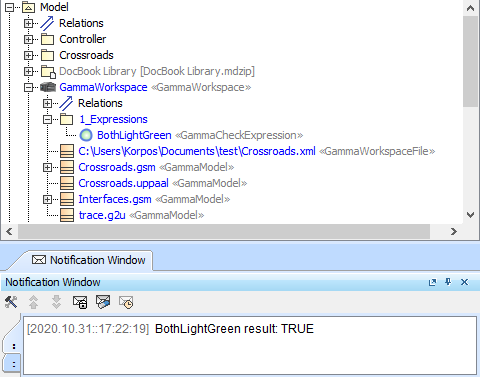
\includegraphics[width=10cm, keepaspectratio]{figures/contribution/verif1.png}
	\caption{Verifikáció futtatásának eredménye}
	\label{fig:verif1}
\end{figure}


Tehát a feltétel teljesül.

%TODO back-annotation, szimuláció

\subsection{Modell javítása}

A problémát úgy lehet kiküszöbölni talán a legkönnyebben, hogy a \emph{Controller}-be is felveszünk egy olyan állapotot amikor várakozik (\ref{fig:fixed} ábra).

\begin{figure}[!ht]
	\centering
	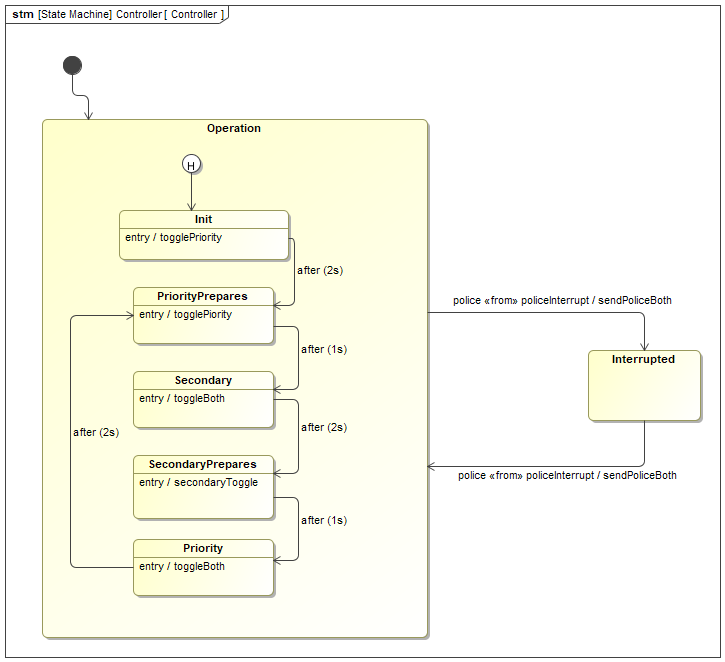
\includegraphics[width=10cm, keepaspectratio]{figures/contribution/ControllerFixed.png}
	\caption{Javított \emph{Controller} állapottérképe}
	\label{fig:fixed}
\end{figure}

A transzformációkat újra végre kell hajtani, hiszen a modell megváltozott. Viszont ha újra futtatjuk a verifikációt akkor már a tulajdonság nem lesz igaz, tehát valóban sikerült javítani a modellt (\ref{fig:verif2} ábra).

\begin{figure}[!ht]
	\centering
	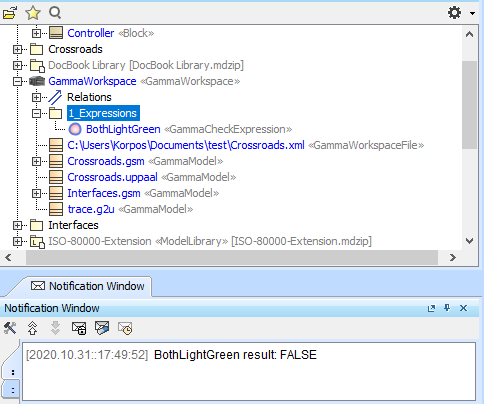
\includegraphics[width=10cm, keepaspectratio]{figures/contribution/verif2.png}
	\caption{Verifikáció futtatásának eredménye a javított modellen}
	\label{fig:verif2}
\end{figure}




